\textbf{Adhäsion:} Ist bestimmt durch stoffliche Wechselwirkungen, durch lokale Pressungen an einzelnen Rauheitshügeln, es entstehen Kaltverschweissungen.\\

\textbf{Abrasion:}\\

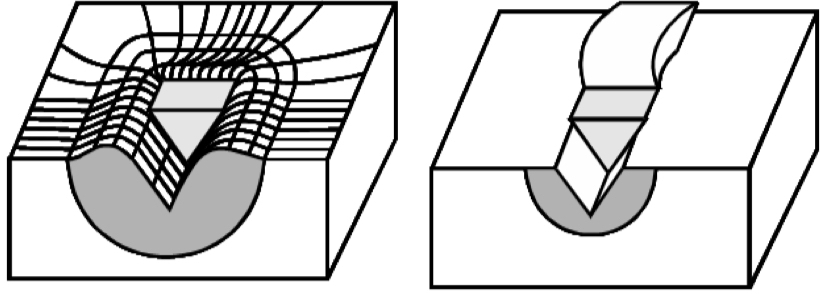
\includegraphics[width=0.5 \linewidth]{src/images/Verschleiss1.jpeg}
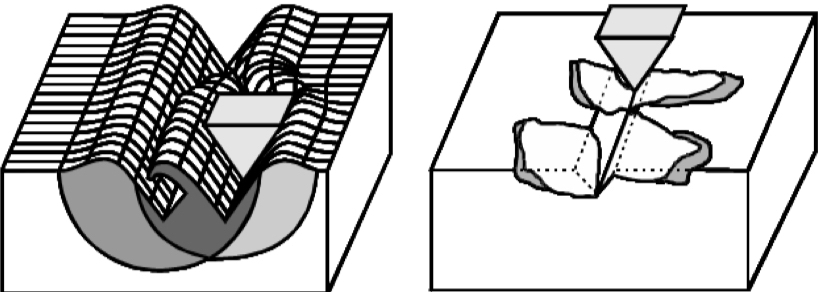
\includegraphics[width=0.5 \linewidth]{src/images/Verschleiss2.jpeg}

Mikropflügen, Mirkrospanen, Mirkoermüden, Mikrobrechen\\


\begin{minipage}{0.5\linewidth}
    \textbf{Verschleiss nach Archard:}\\
    \[
    \boxed{     
        V = k \frac{LF}{3H}
    }
    \]
\end{minipage}
\begin{minipage}{0.5\linewidth}
    \begin{tiny}
    \item $V$: Verschleissvolumen
    \item $k$: Verschleisskoeff.
    \item $L$: Gleitstrecke
    \item $F$: Normalkraft
    \item $H$: Härte
    \end{tiny}
\end{minipage}
\vspace{1mm}

\textbf{Standzeit nach Taylor:}\\
\begin{minipage}{0.5\linewidth}
    \[
    \boxed{     
        T_c = C_v \cdot v_c^k
    }
    \]
\end{minipage}
\begin{minipage}{0.5\linewidth}
    \begin{tiny}
    \item $T_c$: Standzeit
    \item $v_c$: Schnittgeschiwndigkeit
    \item $C_v$ und $k$: Werkzeugspez. Konstante
    \end{tiny}
\end{minipage}\\
\vspace{1mm}
\textbf{Kienze-Gleichung:}\\
\begin{minipage}{0.5\linewidth}
    \[
    \boxed{     
        F_s = \frac{F_c}{b}
    }
    \]
\end{minipage}
\begin{minipage}{0.5\linewidth}
    \begin{tiny}
    \item $F_s$: Spankraft
    \item $F_c$: Schnittkraft
    \item $b$: Schnittbreite/Spanungsbreite
    \end{tiny}
\end{minipage}\\
\vspace{1mm}

\textbf{Stumpfe Werkzeugspitze: }\\
$\uparrow$ Spitzenradius $r_t$ $\not\rightarrow$ $\downarrow$ Schnitttiefe\\
$\uparrow$ Oberflächenspannung, Risse\\
$\uparrow$ Neigung der Aufbauschneidenbildung


